\ffigbox[\FBwidth]{%
\caption{\centering Graphe \(G\) avec 3-cycle \(C\) et un 3-sommet}\label{fig:c3_plus_3}
}{
    \fbox{
        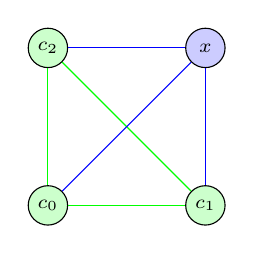
\begin{tikzpicture}[scale=1, main node/.style={circle, draw, fill=blue!20, inner sep=1pt, font=\scriptsize, minimum size=5mm, text=black}]
            % construction de C
            \node[main node, fill=green!20] (c0) at (0, 0) {\(c_0\)};
            \node[main node, fill=green!20] (c1) at (2, 0) {\(c_1\)};
            \node[main node, fill=green!20] (c2) at (0, 2) {\(c_2\)};
            \draw[draw=green] (c0) to (c1);
            \draw[draw=green] (c1) to (c2);
            \draw[draw=green] (c2) to (c0);

            % rajout du 3-sommet
            \node[main node, fill=blue!20] (x) at (2, 2) {\(x\)};
            
            \draw[draw=blue] (x) to (c0);
            \draw[draw=blue] (x) to (c1);
            \draw[draw=blue] (x) to (c2);
        \end{tikzpicture}
    }
}